\documentclass[12pt,a4paper]{article}
\usepackage[utf8]{inputenc}
\usepackage[english]{babel}
\bibliographystyle{unsrt}
\usepackage{amsmath}
\usepackage{amsfonts}
\usepackage{amssymb}
\usepackage{graphicx}
\usepackage{enumitem}
\usepackage{rotating}

\begin{document}
	\section{Description}
	Networks with Virtual Network Functions (VNF) are commonplace today.
	However, the scaling of the system and where to place these VNF efficiently is a still heavy researched subject.
	The goal of this master thesis is to predict the network traffic that requires the network to be scaled and new VNFs to be placed.
	
	The problem with VNFs is that they take some time to start.
	When a system can only react to a request and not predict it, the time for starting the VNF will be added to the waiting time of the request.
	However, if all services are always running at each node, it is a waste of resources, and the fulfilment of a request probably takes extra time since the services take resource from each other.
	The better approach would be to predict the requests so that the system can start the service early to compensate for its startup time.
	
	\section{Motivation}
	The problem with Algorithms like \cite{draxlerScaling} is the fact that they can only react to a request.
	When a service request arrives for a service that was not previously started by the system, the service request must wait the extra startup time.
	The same problem arises when the network has to be scaled to match the incoming requests.
	If the Algorithm determines that the system needs to add a new node to the network, it can only do so after the request already arrived.
	
	The idea of this master thesis is to rectify the problems of the reactive nature of these algorithms.
	For this purpose, the goal is to develop and test machine learning models that can reliably predict new requests and what services are needed.
	With these predictions, an algorithm could then compensate for the startup time of services, shut down services earlier or keep services running if a new request is imminent to arrive.
	The same is true for the scaling of the network.
	
	\section{Gathering Data}
	The first major topic for this master thesis is the research of data for training and testing the models.
	There are multiple sets of data available; two examples are \cite{GoogleData} and \cite{FacebookData} from google and facebook.
	These data sets contain traces from their networks.
	There are also many more sets of traces from other networks.
	
	The first big step will be to download multiple sets of data and sift through them to find the most suitable set.
	The available data is with a high likelihood, not in a good format and is missing data or has too much data.
	The data needs to at least contain the source address, destination address and the time of the request.
	Ideally, the data should also contain the service chain that is associated with the request, but there is probably no data with service chains available.
	However, since a service chain is needed, the data needs to be annotated with an artificial service chain.
	How this chain is determined will also part of the collection and preparation step.
	
	The preparation of the data will be done using R or Python libraries since the amount of data is so high that special data processing libraries are needed.
	Traces could also be generated, but the development of a suitable algorithm to generate realistic traces would probably take an equal amount of time to prepare already existing data.
	Furthermore, using real data increases the credibility of the results of this master thesis.
	
	Also, if the network structure will be used to train the machine learning models, that network has to be modelled.
	If the data doesn't contain the network structure, the network has to be derived.
	Deriving the network structure just from the traces might not be possible and the training must than be done without the network structure.
	
	\section{Model Building}
	The central part of the thesis is the building of the machine learning models.
	To build a machine learning model, multiple libraries exist to abstract the task of creating these models.
	One of the better-known ones is Tensorflow. It is made by Google and uses other machine learning libraries to abstract further the task of creating and training these models. It will be the first library that will be looked at because there exist a large number of tutorials for it and in the Computer cluster of the University of Paderborn exists hardware support for Tensorflow. However, another library I will look at is Keras. Tensorflow uses Keras to build and train Neural Networks and maybe there exist advantages to use the library directly instead of Tensorflow. A short time will also be spent looking at other libraries, but Tensorflow and Keras are the top two choices.
	
	After the library is chosen, the next task is to implement the machine learning models. However, the question is what kind of model should be used. A promising candidate is LSTMs. LSTM, developed in 1995 \cite{lstmOrig}, stands for Long short-term memory. This machine learning model is a neural network, but the weight of each neuron is calculated differently than in the standard neural network. Each neuron has multiple operations to calculate its new weight. However, the essential part of LSTMs is that each neuron considers its previous value. In a sense, it “remembers” what it did before. An LSTM has what regular neural networks are missing; it has a context for what came before the current input data. 
	
	To have a comparison for the more advanced LSTM, a basic Neural Network will also be implemented and tested how well it can predict future requests.
	To have a baseline for the quality of the predictions, an already established model will also be used. This model is the ARIMA model, but it is no machine learning model. The ARIMA model is a statistical model for predicting a time series.
	
	A big part of building the machine learning models is the modelling of the inputs. The most challenging part here will be modelling the current network structure. Typically inputs for a neural network are floating point numbers ranging from 0 to 1. Efficiently mapping a network structure to these inputs is no trivial task. The same problem exists for the source-address, destination-address, service chain, time of request and many more possible attributes.
	
	Also, a question that arises with the modelling of the input data is that of how large the network can get. Theoretical there are no limits to the size of the network but finding a way of modelling the network structure, and other attributes to match that network is not likely. So the result of the master thesis will probably include a restriction on the size of the network.
	
	Also, for each kind of output, a new model is needed. The prediction of the load at a point in time needs a different model then prediction the load over a period of time.
	
	\section{Train and test}
	After building the machine learning models, they need to be trained. The approach for training neural nets used most often is splitting of the test data into two sets. One set is then used to train the model and the other is used to test the quality of the predictions. Exactly how much of the data is sufficient for good predictions depends on the type of prediction so that no accurate prediction can be stated now.
	
	It is possible that the static training and testing do not deliver the wished results for the application of predicting changing network load. If that is the case, training during runtime might deliver a better result. Instead of relying on the pre-runtime training, each new request is used during runtime to train the model continuously.
	
	When the testing of the machine learning and ARIMA models is complete, the data must be compared. The test will have produced a large number of results. These results will be evaluated using R or Python. The comparison that will be made include the accuracy of prediction in the next timestep, how well the quality of the predictions holds for predictions further into the future, how the well the predictions work when predicting over a period of time instead of a point in time. How and what is evaluated must be chosen carfully as it will fundamentally influence what conclusions will be drawn from the thesis.

	\section{Structure of the thesis}
	\begin{enumerate}[label*=\arabic*.]
		\item Structure of the thesis
	\end{enumerate}
	\section{Timetable}
\begin{sidewaysfigure}
	\centering
	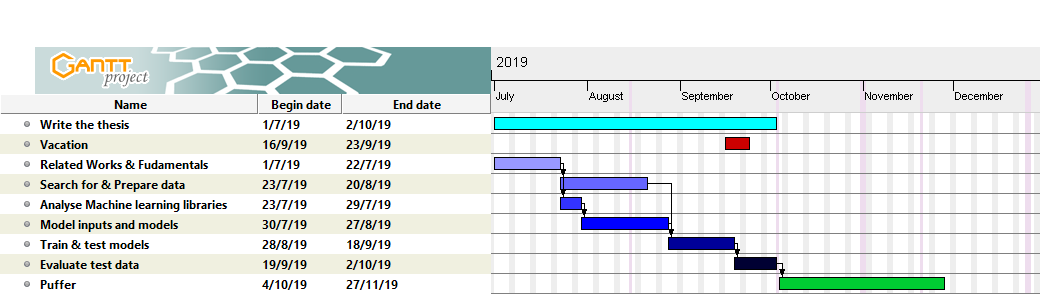
\includegraphics[width=1.0\linewidth]{Timetable/Timetable}
	\caption{}
	\label{fig:timetable}
\end{sidewaysfigure}

\bibliography{proposalBib}


\end{document}